\documentclass[10pt]{article}
\usepackage[a4paper]{geometry}
\usepackage{fullpage}
\usepackage[T1]{fontenc}
\usepackage[utf8]{inputenc}
\usepackage{graphicx}
\usepackage{mathpazo}
\pagenumbering{gobble}
\usepackage{siunitx}
\DeclareSIUnit\voltampere{VA}
\DeclareSIUnit\kWh{kWh}
\usepackage{amsmath}
\usepackage[spanish]{babel}
\usepackage{steinmetz}
\usepackage{diffcoeff}

\renewcommand{\thesection}{Problema \arabic{section}}

\begin{document}

\title{}

\date{Curso 2020-21}

\section{}

Un generador cuya fuerza electromotriz es de \SI{120}{V} y resistencia interna \SI{0.2}{\ohm}, entrega una corriente de \SI{20}{\ampere} a un motor situado a \SI{300}{\meter} de distancia y de resistencia interna \SI{0.5}{\ohm}. La línea es de cobre de resistividad $\SI{17.24}{\milli\ohm\milli\meter\squared\per\meter}$. Sabiendo que el motor absorbe \SI{10.2}{\kWh} en 5 horas, hallar: 
\begin{enumerate}
\item Fuerza contraelectromotriz del motor.
\item Sección de los conductores.
\item Rendimiento del motor, del generador, de la línea y rendimiento total.
\item Balance general de potencias.
\end{enumerate}

\section{}
Un generador de corriente continua alimenta a dos cargas. La primera está situada a \SI{2100}{\meter}, tiene una resistencia de \SI{215}{\ohm} y rendimiento unidad. La segunda está situada a \SI{270}{\meter} después de la primera, tiene una potencia de \SI{4662}{\watt}, un rendimiento del 75\%, y una tensión aplicada de \SI{420}{\volt}.

Sabiendo que la línea es de cobre, de \SI{6}{\milli\meter\squared} de sección, y que la resistividad es de $\SI{17.24}{\milli\ohm\milli\meter\squared\per\meter}$, determinar:

\begin{enumerate}
\item Tensión en bornes del generador.
\item Intensidad entregada por el generador.
\item Rendimiento de la instalación.
\end{enumerate}

\section{}

Convierte en fuente de tensión o intensidad, según corresponda.

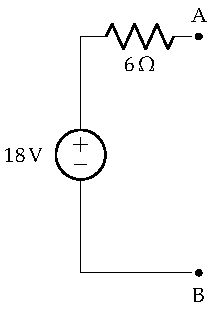
\includegraphics[scale=0.75]{figs/Conversion_Fuentes.pdf}
\hspace{1cm}
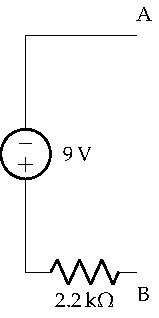
\includegraphics[scale=0.75]{figs/Conversion_Fuentes_2.pdf}
\hspace{1cm}
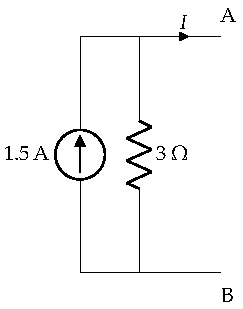
\includegraphics[scale=0.75]{figs/Conversion_Fuentes_3.pdf}
\hspace{1cm}
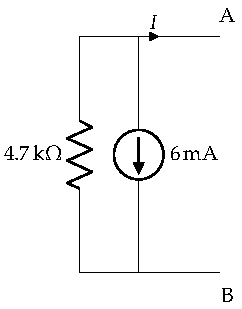
\includegraphics[scale=0.75]{figs/Conversion_Fuentes_4.pdf}

\section{}

\begin{minipage}{0.5\linewidth}
Calcula la resistencia equivalente entre A y B.
\end{minipage}
\begin{minipage}{0.5\linewidth}
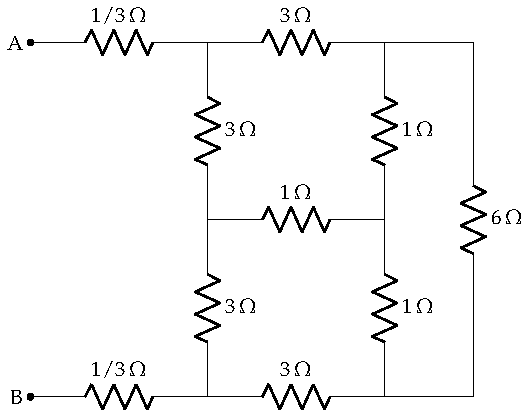
\includegraphics[scale=0.7]{figs/CircuitoResistivo_FM.pdf}
\end{minipage}

\clearpage

\section{}

Analiza el circuito de la figura mediante el método de las mallas, obteniendo:
\begin{enumerate}
\item Corriente de cada una de las ramas
\item Potencial en cada uno de los nudos, tomando como referencia el
  nudo A.
\end{enumerate}

Con estos resultados, realiza un balance de potencias comparando la potencia de los elementos activos y la de los elementos pasivos.

\begin{minipage}{0.4\linewidth}
  Datos:
  \begin{align*}
    R_1 = R_3 = R_6 &= \SI{3}{\ohm}\\
    R_2 = R_4 = R_5 &= \SI{2}{\ohm}\\
    \epsilon_1 &= \SI{245}{\volt}\\
    \epsilon_2 &= \SI{490}{\volt}\\
    \epsilon_3 &= \SI{735}{\volt}\\
  \end{align*}
\end{minipage}
\begin{minipage}{0.6\linewidth}
  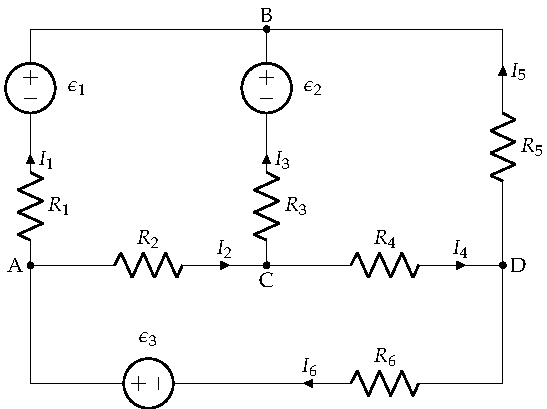
\includegraphics{figs/mallas1.pdf}
\end{minipage}

\subsection*{Solución}

Tal y como se muestra en la figura, usamos tres corrientes de malla dextrógiras. 

  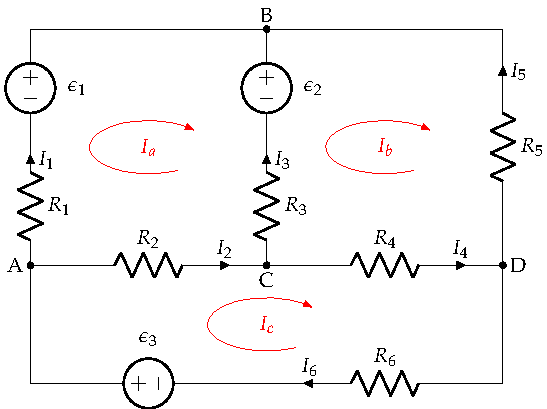
\includegraphics{figs/mallas1_corrientes.pdf}

En primer lugar, establecemos las relaciones entre las corrientes de rama y las corrientes de malla:

\begin{align*}
  I_1 &= I_a\\
  I_2 &= -I_a + I_c\\
  I_3 &= -I_a + I_b\\
  I_4 &= -I_b + I_c\\
  I_5 &= -I_b\\
  I_6 &= I_c
\end{align*}

A continuación, escribimos las ecuaciones del método de las mallas:
\begin{equation*}
  \begin{pmatrix}
    (R_1 + R_3 + R_2) &  - R_3 & - R_2 \\
    - R_3 & (R_5 + R_4 + R_3) & - R_4 \\
    - R_2 & - R_4 &  (R_2 + R_4 + R_6)
  \end{pmatrix} \cdot %
  \begin{pmatrix}
    I_a\\
    I_b\\
    I_c\\
  \end{pmatrix} = %
  \begin{pmatrix}
    \epsilon_1 - \epsilon_2\\
    \epsilon_2\\
    \epsilon_3
  \end{pmatrix}
\end{equation*}

\[
  \left(\begin{array}{ccc}
          8 & -3 & -2 \\
          -3 & 7 & -2 \\
          -2 & -2 & 7\\
        \end{array}\right)%
      \cdot \left(\begin{array}{c}
              I_a\\
              I_b\\
              I_c\\
            \end{array}\right)%
            = \left(\begin{array}{c}
              -245\\
              490\\
              735
            \end{array}\right)
\]
cuya solución es:

\begin{align*}
  I_a &= \SI{65}{\ampere}\\
  I_b &= \SI{145}{\ampere}\\
  I_c &= \SI{165}{\ampere}
\end{align*}

Por tanto, los valores de las corrientes de rama son:

\begin{align*}
  I_1 &= \SI{65}{\ampere}\\
  I_2 &= \SI{100}{\ampere}\\
  I_3 &= \SI{80}{\ampere}\\
  I_4 &= \SI{20}{\ampere}\\
  I_5 &= \SI{-145}{\ampere}\\
  I_6 &= \SI{165}{\ampere}
\end{align*}

Se puede (y se debe) comprobar que estos resultados cumplen la LKC en los nudos del circuito.

Los potenciales en cada punto son, tomando el punto A como referencia:

\begin{align*}
  V_A &= \SI{0}{\volt}\\
  V_B &= U_{BA} = \epsilon_1 - I_1 \cdot R_1 = \SI{50}{\volt}\\
  V_C &= U_{CA} = - I_2 \cdot R_2 = \SI{-200}{\volt}\\
  V_D &= U_{DA} = -I_4 \cdot R_4 + V_D = \SI{-240}{\volt}
\end{align*}


La potencia entregada por los generadores del circuito es:

\begin{align*}
  P_{\epsilon_1} &= \epsilon_1 \cdot I_1 = \SI{15.925}{\kilo\watt}\\
  P_{\epsilon_2} &= \epsilon_2 \cdot I_3 = \SI{39.2}{\kilo\watt}\\
  P_{\epsilon_3} &= \epsilon_3 \cdot I_5 = \SI{121.275}{\kilo\watt}\\
  P_\epsilon &= P_{\epsilon_1} + P_{\epsilon_2} + P_{\epsilon_3} = \SI{176.4}{\kilo\watt}  
\end{align*}

La potencia disipada por las resistencias es:

\begin{align*}
  P_{R_1} &= I_1^2 \cdot R_1 = \SI{12.675}{\kilo\watt}\\
  P_{R_2} &= I_2^2 \cdot R_2 = \SI{20}{\kilo\watt}\\
  P_{R_3} &= I_3^2 \cdot R_3 = \SI{19.2}{\kilo\watt}\\
  P_{R_4} &= I_4^2 \cdot R_4 = \SI{800}{\watt}\\
  P_{R_5} &= I_5^2 \cdot R_5 = \SI{42.05}{\kilo\watt}\\
  P_{R_6} &= I_5^2 \cdot R_5 = \SI{81.675}{\kilo\watt}\\
  P_R &= \sum_i P_{Ri} = \SI{176.4}{\kilo\watt}  
\end{align*}

Comprobamos que se cumple el balance de potencias.

\clearpage

\section{}
Analiza el circuito de la figura mediante el método de las mallas, obteniendo la corriente de cada una de las ramas. Con este resultado calcula la diferencia de potencial entre A y B, y realiza un balance de potencias comparando la potencia de los elementos activos y la de los elementos pasivos.

\begin{minipage}{0.4\linewidth}
  Datos:
  \begin{align*}
    R_1 = R_2 &= \SI{1}{\ohm}\\
    R_3 &= \SI{2}{\ohm}\\
    R_4 &= \SI{3}{\ohm}\\
    R_5 &= \SI{4}{\ohm}\\
    \epsilon_1 &= \SI{118}{\volt}\\
    \epsilon_2 &= \SI{236}{\volt}\\
    \epsilon_3 &= \SI{118}{\volt}\\
  \end{align*}
\end{minipage}
\begin{minipage}{0.6\linewidth}
  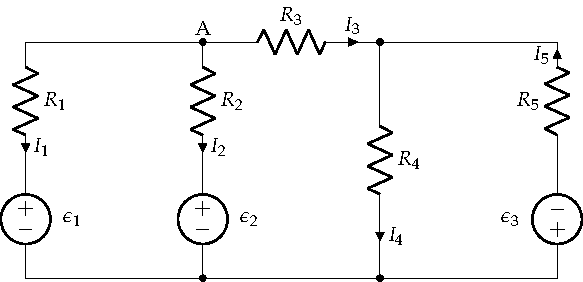
\includegraphics{figs/mallas2.pdf}
\end{minipage}

\subsection*{Solución}

Como es habitual, usaremos tres corrientes de malla dextrógiras. Las nombramos de izquierda a derecha, $I_a$, $I_b$ e $I_c$.

En primer lugar, establecemos las relaciones entre las corrientes de rama y las corrientes de malla:

\begin{align*}
  I_1 &= -I_a\\
  I_2 &= I_a - I_b\\
  I_3 &= I_b\\
  I_4 &= I_b - I_c\\
  I_5 &= I_c
\end{align*}

A continuación, escribimos las ecuaciones del método de las mallas:

\[
  \left(\begin{array}{ccc}
          R_1 + R_2 & -R_2 & 0\\
          -R_2 & R_2 + R_3 + R_4 & - R_4\\
          0 & -R_4 & R_4 + R_5\\
        \end{array}\right)%
      \cdot \left(\begin{array}{c}
              I_a\\
              I_b\\
              I_c\\
            \end{array}\right)%
            = \left(\begin{array}{c}
              \epsilon_1 - \epsilon_2\\
              \epsilon_2\\
              \epsilon_3
            \end{array}\right)
\]

\[
  \left(\begin{array}{ccc}
          2 & -1 & 0 \\
          -1 & 6 & -3 \\
          0 & -3 & 7\\
        \end{array}\right)%
      \cdot \left(\begin{array}{c}
              I_a\\
              I_b\\
              I_c\\
            \end{array}\right)%
            = \left(\begin{array}{c}
              -118\\
              236\\
              118
            \end{array}\right)
\]
cuya solución es:

\begin{align*}
  I_a &= \SI{-32}{\ampere}\\
  I_b &= \SI{54}{\ampere}\\
  I_c &= \SI{40}{\ampere}
\end{align*}

Por tanto, los valores de las corrientes de rama son:

\begin{align*}
  I_1 &= \SI{32}{\ampere}\\
  I_2 &= \SI{-86}{\ampere}\\
  I_3 &= \SI{54}{\ampere}\\
  I_4 &= \SI{14}{\ampere}\\
  I_5 &= \SI{40}{\ampere}
\end{align*}

Se puede (y se debe) comprobar que estos resultados cumplen la LKC en los nudos del circuito.

La diferencia de potencial entre A y B es:

\[
  U_{AB} = I_3 \cdot R_3 + I_4 \cdot R_4 = \SI{150}{\volt}
\]

La potencia entregada por los generadores del circuito es:

\begin{align*}
  P_{\epsilon_1} &= \epsilon_1 \cdot (-I_1) = -\SI{3,776}{\kilo\watt}\\
  P_{\epsilon_2} &= \epsilon_2 \cdot (-I_2) = \SI{20,296}{\kilo\watt}\\
  P_{\epsilon_3} &= \epsilon_3 \cdot I_5 = \SI{4,72}{\kilo\watt}\\
  P_\epsilon &= P_{\epsilon_1} + P_{\epsilon_2} + P_{\epsilon_3} = \SI{21,42}{\kilo\watt}  
\end{align*}

Es importante recordar que el criterio de signos de un generador considera que la potencia entregada es positiva cuando la corriente sale del generador por su terminal positivo. Por tanto, $I_1$ e $I_2$ son empleadas con un signo negativo. En consecuencia, la potencia del generador $\epsilon_1$ es negativa, lo que quiere decir que este generador funciona como receptor (absorbe potencia) Ahora bien, dado que $I_2$ tiene valor negativo (es decir, circula en sentido contrario al indicado en la figura), la potencia del generador $\epsilon_2$ es positiva, de forma que este generador actúa como tal.

La potencia disipada por las resistencias es:

\begin{align*}
  P_{R_1} &= I_1^2 \cdot R_1 = \SI{1,024}{\kilo\watt}\\
  P_{R_2} &= I_2^2 \cdot R_2 = \SI{7,396}{\kilo\watt}\\
  P_{R_3} &= I_3^2 \cdot R_3 = \SI{5,832}{\kilo\watt}\\
  P_{R_4} &= I_4^2 \cdot R_4 = \SI{588}{\watt}\\
  P_{R_5} &= I_5^2 \cdot R_5 = \SI{6,4}{\kilo\watt}\\
  P_R &= \sum_i P_{Ri} = \SI{21,42}{\kilo\watt}  
\end{align*}

Comprobamos que se cumple el balance de potencias.

\clearpage

\section{}

En el circuito de la figura se debe emplear el método de los nudos para determinar:
\begin{itemize}
\item Las tensiones en los nudos A y B.
\item Las corrientes de todas las ramas.
\item El balance de potencias, diferenciando entre elementos activos y elementos pasivos.
\end{itemize}

\begin{minipage}[c]{0.3\linewidth}
  \begin{align*}
    \epsilon_1&=\SI{6}{\volt}\\
    \epsilon_2&=\SI{12}{\volt}\\
    \epsilon_3&=\SI{24}{\volt}\\
    I_{g1} &= \SI{15}{\ampere}\\
    I_{g2} &= \SI{9}{\ampere}\\
    I_{g3} &= \SI{6}{\ampere}\\
    R_{1}&= R_3 = R_4 = R_5 = \SI{2}{\ohm}\\
    R_{2}&= \SI{1}{\ohm}
  \end{align*}
\end{minipage}
\begin{minipage}[c]{0.7\linewidth}
  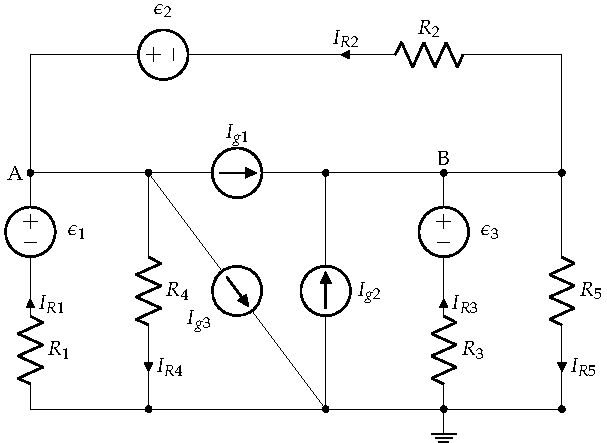
\includegraphics{figs/nudos_fuentes.pdf}
\end{minipage}

\subsection*{Solución}


Transformando las fuentes de tensión en fuentes de corriente obtenemos:

\[
\small{
\left(\begin{array}{ccc}
    1/R_1 + 1/R_2 + 1/R_4 & -1/R_2\\
    -1/R_2 & 1/R_2 + 1/R_3 + 1/R_5
  \end{array}\right) \cdot \left(\begin{array}{c}
    V_{A}\\
    V_{B}
  \end{array}\right) = 
\left(\begin{array}{c}
        E_1/R_1 + E_2/R_2 - I_1 - I_3\\
        -E_2/R_2 + I_1 + I_2 + E_3/R_3
      \end{array}\right)
  }
\]

La solución de esta ecuación matricial es $V_A = \SI{4}{\volt}$ y $V_B = \SI{14}{\volt}$. 

Con estos resultados podemos calcular las corrientes que circulan por las resistencias asociadas a los generadores de tensión:

\begin{align*}
V_A &= E_1 - I_{R1} R_1\\
V_{AB} &= E_2 - I_{R2} R_2\\
V_B &= E_3 - I_{R3} R_3\\
\end{align*}

\begin{align*}
I_{R1} &= \SI{1}{\ampere}\\
I_{R2} &= \SI{22}{\ampere}\\
I_{R3} &= \SI{5}{\ampere}
\end{align*}

Por tanto, los elementos activos aportan un total de \SI{642}{\watt}:

\begin{align*}
P_{I1} &= I_1 V_{BA} = \SI{150}{\watt}\\
P_{I2} &= I_2 V_{B} = \SI{126}{\watt}\\
P_{I1} &= I_3 (-V_{A}) = - \SI{24}{\watt}\\
P_{E1} &= E_1 I_{R1} = \SI{6}{\watt}\\
P_{E2} &= E_2 I_{R2} = \SI{264}{\watt}\\
P_{E3} &= E_3 I_{R3} = \SI{120}{\watt}
\end{align*}

Los elementos pasivos consumen un total de \SI{642}{\watt}:

\begin{align*}
P_{R1} &= I^2_{R1} R_1 = \SI{2}{\watt}\\
P_{R2} &= I^2_{R2} R_2 = \SI{484}{\watt}\\
P_{R3} &= I^2_{R3} R_3 = \SI{50}{\watt}\\
P_{R4} &= I^2_{R4} R_4 = \SI{8}{\watt}\\
P_{R5} &= I^2_{R5} R_5 = \SI{98}{\watt}
\end{align*}

\clearpage

\section{}
Aplica el método de los nudos en el circuito de la figura para determinar:
\begin{enumerate}
\item Los potenciales de los nudos A, B, C y D.
\item Las intensidades de corriente señaladas.
\item Carga, polaridad y energía almacenada en los condensadores,
  supuestos sin carga inicial.
\end{enumerate}

\begin{minipage}[c]{0.3\textwidth}
  \begin{align*}
    R_i &= \mathrm{i\ } \si{\ohm}\\
    C_i &= \mathrm{i\ } \si{\micro\farad}\\
    E_1 &= \SI{6}{\volt}\\
    E_2 &= \SI{18}{\volt}\\
    E_3 &= \SI{6}{\volt}\\
  \end{align*}
\end{minipage}
\begin{minipage}[c]{0.7\textwidth}
  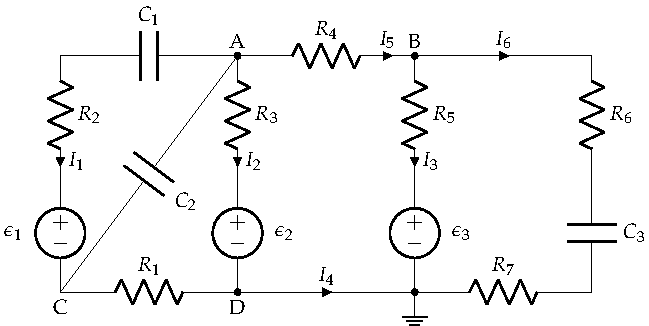
\includegraphics[width=\textwidth]{figs/nudos_condensadores.pdf}
\end{minipage}

\subsection*{Solución}

Sustituimos los condensadores por circuitos abiertos. En consecuencia, por las ramas correspondientes no puede circular corriente. En particular:

\begin{align*}
  I_1 &= \SI{0}{\ampere}\\
  I_6 &= \SI{0}{\ampere}
\end{align*}

Para aplicar el método de los nudos transformamos las fuentes $\epsilon_2$ y $\epsilon_3$ en fuentes de corriente. Las ecuaciones del método de los nudos son:

\begin{equation*}
  \begin{bmatrix}
    G_3 + G_4 & -G_4\\
    -G_4 & G_5 + G_4\\
  \end{bmatrix} \cdot %
  \begin{bmatrix}
    V_A\\
    V_B
  \end{bmatrix} = %
  \begin{bmatrix}
    \epsilon_2/R_3\\
    \epsilon_3/R_5
  \end{bmatrix}
\end{equation*}

Sustituimos valores y resolvemos:

\begin{align*}
  V_A &= \SI{15}{\volt}\\
  V_B &= \SI{11}{\volt}
\end{align*}

Además, $V_D = 0$, dado que está conectado a tierra. Por otra parte, la caída de tensión en la resistencia $R_1$ es 0 porque $I_1 = 0$, luego $V_C = V_D$.

Con estos resultados podemos obtener los valores de las corrientes de rama. Volvemos al circuito original para plantear las ecuaciones de rama:

\begin{align*}
  V_A &= I_2 \cdot R_3 + \epsilon_2\\
  V_B &= I_3 \cdot R_5 + \epsilon_3
\end{align*}

De estas ecuaciones despejamos $I_2$ e $I_3$. Además, teniendo en cuenta que $I_1 = I_6 = 0$, tenemos:

\begin{align*}
  I_5 &= I_3\\
  I_4 &= I_2\\
  I_2 &= -I_3
\end{align*}

En definitiva:

\begin{align*}
  I_1 &= \SI{0}{\ampere}\\
  I_2 &= \SI{-1}{\ampere}\\
  I_3 &= \SI{1}{\ampere}\\
  I_4 &= \SI{-1}{\ampere}\\
  I_5 &= \SI{1}{\ampere}\\
  I_6 &= \SI{0}{\ampere}
\end{align*}

Finalmente, calculamos las diferencias de potencial en los
condensadores. En $C_1$ asignamos la polaridad positiva en A, y
tenemos:

\begin{equation*}
  U_{AC} = U_{C1} + \epsilon_1 \rightarrow U_{C1} = \SI{9}{\volt}
\end{equation*}

Para $C_2$ y $C_3$ el cálculo es directo, asignando la polaridad positiva en A y B, respectivamente:

\begin{align*}
  U_{C2} &=  U_{AC} = \SI{15}{\volt}\\
  U_{C3} &=  U_{BD} = \SI{11}{\volt}
\end{align*}

En consecuencia, las cargas almacenadas en cada condensador son:

\begin{align*}
  q_1 &= C_1 \cdot U_{C1} = \SI{9}{\micro\coulomb}\\
  q_2 &= C_2 \cdot U_{C2} = \SI{30}{\micro\coulomb}\\
  q_3 &= C_3 \cdot U_{C3} = \SI{33}{\micro\coulomb}
\end{align*}

Y las energías:

\begin{align*}
  E_{C1} &= \frac{1}{2} \cdot C_1 \cdot U^2_{C1} = \SI{40.5}{\micro\joule}\\
  E_{C2} &= \frac{1}{2} \cdot C_2 \cdot U^2_{C2} = \SI{225}{\micro\joule}\\
  E_{C3} &= \frac{1}{2} \cdot C_3 \cdot U^2_{C3} = \SI{181.5}{\micro\joule}
\end{align*}


\clearpage

\section{}

En el circuito de la figura debes determinar:
\begin{itemize}
\item Las intensidades señaladas.
\item Los potenciales en los puntos A, B, C, D, E y F.
\end{itemize}


\begin{minipage}[c]{0.2\linewidth}
  \begin{align*}
    \epsilon_{A}&=\SI{90}{\volt}\\
    \epsilon_{B}&=\SI{60}{\volt}\\
    \epsilon_{C}&=\SI{30}{\volt}\\
    R_{1}&= R_2 = R_3 = \SI{10}{\ohm}\\
    R_{4}&= R_5 = \SI{30}{\ohm}\\
    C_{1}&= \SI{10}{\micro\farad}\\
    C_{2}&= \SI{20}{\micro\farad}\\
    L_1 &= \SI{1}{\micro\henry}\\
    q^0_{C1} &= \SI{10}{\micro\coulomb}\\
    q^0_{C2} &= \SI{20}{\micro\coulomb}
  \end{align*}
\end{minipage}
\begin{minipage}[c]{0.8\linewidth}
  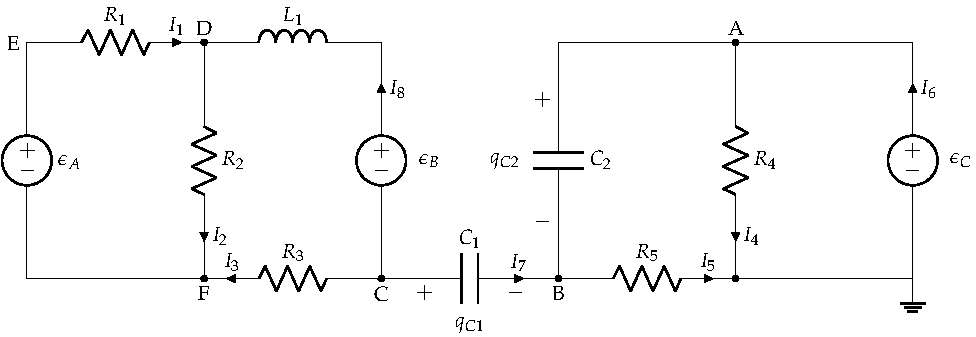
\includegraphics[scale = 0.8]{figs/mallas_carga_inicial.pdf}
\end{minipage}

\subsection*{Solución}

Sustituimos los condensadores por circuitos abiertos. En consecuencia, por las ramas correspondientes no puede circular corriente. En particular:

\begin{align*}
  I_5 &= \SI{0}{\ampere}\\
  I_7 &= \SI{0}{\ampere}
\end{align*}

En consecuencia,

\begin{align*}
  I_3 &= -I_8\\
  I_4 &= I_6
\end{align*}

Además, la bobina $L_1$ es un cortocircuito.

En el circuito de la izquierda tenemos dos mallas, y definimos dos corrientes de malla dextrógiras:

\begin{equation*}
  \begin{bmatrix}
    R_1 + R_2 & -R_2\\
    -R_2 & R_2 + R_3\\
  \end{bmatrix} \cdot %
  \begin{bmatrix}
    I_a\\
    I_b
  \end{bmatrix} = %
  \begin{bmatrix}
    \epsilon_A\\
    -\epsilon_B
  \end{bmatrix}
\end{equation*}

La solución de este sistema es:

\begin{align*}
  I_a &= \SI{4}{\ampere}\\
  I_b &= \SI{-1}{\ampere}
\end{align*}
siendo,

\begin{align*}
  I_1 &= I_a\\
  I_2 &= I_a - I_b\\
  I_3 &= I_b\\
  I_8 &= -I_b
\end{align*}

Para el circuito de la derecha tenemos una única malla:

\begin{equation*}
  \epsilon_C = I_4 \cdot R_4 \rightarrow I_4 = \SI{1}{\ampere}
\end{equation*}

Por tanto,

\begin{align*}
  I_1 &= \SI{4}{\ampere}\\
  I_2 &= \SI{5}{\ampere}\\
  I_3 &= \SI{-1}{\ampere}\\
  I_4 &= \SI{1}{\ampere}\\
  I_5 &= \SI{0}{\ampere}\\
  I_6 &= \SI{1}{\ampere}\\
  I_7 &= \SI{0}{\ampere}\\
  I_8 &= \SI{1}{\ampere}\\
\end{align*}

Los potenciales en los puntos A y B se calculan así:

\begin{align*}
  V_A &= \epsilon_C = \SI{30}{\volt}\\
  V_B &= R_5 \cdot I_5 = \SI{0}{\volt}
\end{align*}

Para calcular el potencial en el punto C debemos tener en cuenta que el condensador $C_1$ conserva su carga inicial porque el circuito no está cerrado en la parte superior. Por tanto,

\begin{equation*}
  U_{CB} = U_{C1} = \frac{q^0_{C1} }{C_1} = \SI{1}{\volt}
\end{equation*}

Por tanto,

\begin{equation*}
  U_C = U_{CB} + U_B = \SI{1}{\volt}
\end{equation*}

A partir de este resultado podemos calcular el resto de potenciales:

\begin{align*}
  U_D &= U_{DC} + U_C = \epsilon_B + U_C = \SI{61}{\volt}\\
  U_E &= U_{ED} + U_D = I_1 \cdot R_1 + U_D = \SI{101}{\volt}\\
  U_F &= U_{FC} + U_C = -I_3 \cdot R_3 + U_C = \SI{11}{\volt}
\end{align*}

\clearpage

\section{}

En el esquema de la figura los condensadores se conectaron sin
carga. Mediante el método de las mallas determina:
\begin{enumerate}
\item Intensidades de corriente señaladas.
\item Potenciales en los puntos A, B, C y D.
\item Polaridades, cargas, y energías de los condensadores.
\item Balance de potencias.
\end{enumerate}

\begin{minipage}[c]{0.3\linewidth}
  \begin{align*}
    \epsilon_{1}&=\SI{118}{\volt}\\
    \epsilon_{2}&=\SI{236}{\volt}\\
    \epsilon_{3}&=\SI{118}{\volt}\\
    R_{1}&= \SI{4}{\ohm}\\
    R_{2}&=R_{3}=\SI{1}{\ohm}\\
    R_{4}&= \SI{3}{\ohm}\\
    R_{5}&= \SI{2}{\ohm}\\
    C_{1}&=C_{2}=C_{3}=\SI{2}{\micro\farad}\\
    X_1 &= X_2 = X_3 = \SI{1}{\ohm}\\
  \end{align*}
\end{minipage}
\begin{minipage}[c]{0.7\linewidth}
  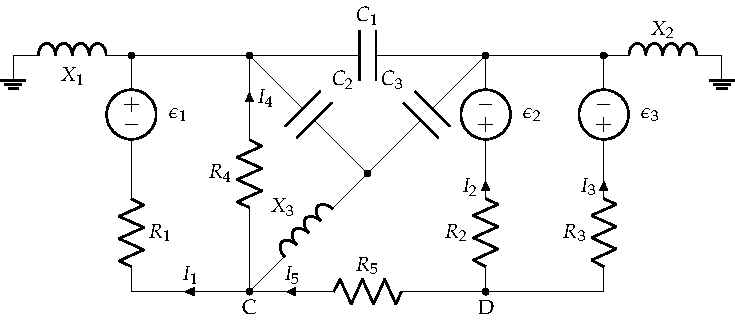
\includegraphics{figs/mallas_condensadores.pdf}
\end{minipage}

\subsection*{Solución}
Sustituimos los condensadores y las bobinas por sus equivalentes en un circuito de corriente continua. En el circuito resultante marcamos tres corrientes de malla dextrógiras, y planteamos la matriz correspondiente para resolver por mallas: 

\[
\small{
\left(\begin{array}{c}
    E_1\\
    E_2\\
    E_3 - E_2
  \end{array}\right) = \left(\begin{array}{ccc}
    R_1 + R_4 & -R_4 & 0\\
    -R_4 & R_4 + R_5 + R_2 & -R_{2}\\
    0 & -R_2 & R_2 + R_3
  \end{array}\right) \cdot \left(\begin{array}{c}
    I_{A}\\
    I_{B}\\
    I_{C}
  \end{array}\right)
}
\]

\[
\small{
\left(\begin{array}{c}
    118\\
    236\\
    118
  \end{array}\right) = \left(\begin{array}{ccc}
    7 & -3 & 0\\
    -3 & 6 & -1\\
    0 & -1 & 2
  \end{array}\right) \cdot \left(\begin{array}{c}
    I_{A}\\
    I_{B}\\
    I_{C}
  \end{array}\right)
}
\]

La solución es:

\begin{eqnarray*}
I_A & = & \SI{40}{\ampere}\\
I_B & = & \SI{54}{\ampere}\\
I_C & = & -\SI{32}{\ampere}
\end{eqnarray*}

Por tanto, las corrientes indicadas en el circuito son:

\begin{eqnarray*}
I_1 & = & \SI{40}{\ampere}\\
I_2 & = & \SI{-86}{\ampere}\\
I_3 & = &  \SI{32}{\ampere}\\
I_4 & = &  \SI{14}{\ampere}\\
I_5 & = &  \SI{54}{\ampere}
\end{eqnarray*}

Las tensiones en los puntos indicados son:

\begin{align*}
V_A &= \SI{0}{\volt}\\
V_B &= \SI{0}{\volt}\\
V_C &= I_4 \cdot R_4 = \SI{42}{\volt}\\
V_D &= I_5 \cdot R_5 + V_c = \SI{150}{\volt}\\
\end{align*}

Por tanto, las polaridades de los condensadores son las marcadas en la figura, con los valores de tensión siguientes:

\begin{eqnarray*}
U_{C1} = U_{BA} & = & \SI{0}{\volt}\\
q_1 = C_1 \cdot U_{C1} & = & \SI{0}{\micro\coulomb}\\
E_{C2} & = & \SI{0}{\joule}
\end{eqnarray*}

\begin{eqnarray*}
U_{C2} = U_{CA} & = & \SI{42}{\volt}\\
q_2 = C_2 \cdot U_{C2} & = & \SI{84}{\micro\coulomb}\\
E_{C2} & = & \SI{1.76}{\milli\joule}
\end{eqnarray*}

\begin{eqnarray*}
U_{C3} = U_{CB} & = & \SI{42}{\volt}\\
q_3 = C_3 \cdot U_{C3} & = & \SI{84}{\micro\coulomb}\\
E_{C3} & = & \SI{1.76}{\milli\joule}
\end{eqnarray*}

Finalmente, el balance de potencias calcula la potencia entregada por los elementos activos y la potencia consumida por los elementos pasivos.

La potencia total entregada por los elementos activos es $\SI{21240}{\watt}$:
\begin{eqnarray*}
P_{E1} = E_1 \cdot I_1 & = & \SI{4720}{\watt}\\
P_{E2} = E_2 \cdot (-I_2) & = & \SI{20296}{\watt}\\
P_{E3} = E_3 \cdot (-I_3) & = & \SI{-3776}{\watt}
\end{eqnarray*}

La potencia total consumida por los elementos pasivos también es $\SI{21240}{\watt}$:
\begin{eqnarray*}
P_{R1} = R_1 \cdot I_1^2 & = & \SI{6400}{\watt}\\
P_{R2} = R_2 \cdot I_2^2 & = & \SI{7396}{\watt}\\
P_{R3} = R_3 \cdot I_3^2 & = & \SI{1024}{\watt}\\
P_{R4} = R_4 \cdot I_4^2 & = & \SI{588}{\watt}\\
P_{R5} = R_5 \cdot I_5^2 & = & \SI{5832}{\watt}
\end{eqnarray*}

\clearpage

\section{}

En el circuito de la figura se debe determinar:
\begin{itemize}
\item Las corrientes señaladas.
\item El balance de potencias, diferenciando entre elementos activos y elementos pasivos.
\item Los potenciales en los puntos A, B y C.
\item La carga, polaridad y energía almacenada en los condensadores, supuestos sin carga inicial.
\end{itemize}

\begin{minipage}[c]{0.3\linewidth}
  \begin{align*}
    \epsilon_1&=\SI{1}{\volt}\\
    \epsilon_2&=\SI{7}{\volt}\\
    R_i &= \SI{1}{\ohm}\\
    C_i &= \SI{i}{\micro\farad}
  \end{align*}
\end{minipage}
\begin{minipage}[c]{0.7\linewidth}
  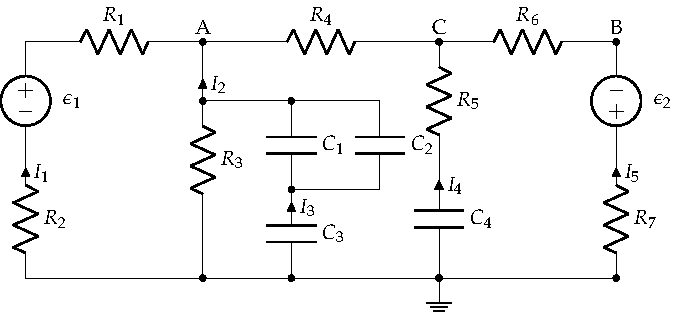
\includegraphics{figs/mallas_agrupacion_condensadores.pdf}
\end{minipage}

\subsection*{Solución}

Sustituimos los condensadores por circuitos abiertos. En consecuencia, por las ramas correspondientes no puede circular corriente. En particular:

\begin{align*}
  I_3 &= \SI{0}{\ampere}\\
  I_4 &= \SI{0}{\ampere}
\end{align*}

Tenemos dos mallas, y definimos dos corrientes de malla dextrógiras:

\begin{equation*}
  \begin{bmatrix}
    R_1 + R_2 + R_3 & -R_3\\
    -R_3 & R_3 + R_4 + R_6 + R_7\\
  \end{bmatrix} \cdot %
  \begin{bmatrix}
    I_a\\
    I_b
  \end{bmatrix} = %
  \begin{bmatrix}
    \epsilon_1\\
    \epsilon_2
  \end{bmatrix}
\end{equation*}

La solución de este sistema es:

\begin{align*}
  I_a &= \SI{1}{\ampere}\\
  I_b &= \SI{2}{\ampere}
\end{align*}
siendo,

\begin{align*}
  I_1 &= I_a = \SI{1}{\ampere}\\
  I_2 &= I_b - I_a = \SI{1}{\ampere}\\
  I_5 &= -I_b = \SI{-2}{\ampere}
\end{align*}

La potencia de los dos elementos activos es:

\begin{align*}
  P_{\epsilon1} = \epsilon_1 \cdot I_1 = \SI{1}{\watt}\\
  P_{\epsilon2} = \epsilon_2 \cdot (-I_5) = \SI{14}{\watt}
\end{align*}

En total, $P_\epsilon = \SI{15}{\watt}$.

Aplicando la ley de Joule en cada resistencia comprobamos que la potencia total disipada en las resistencias del circuito coincide con esta cantidad.

Los potenciales en los puntos indicados son:

\begin{align*}
  V_A &= -I_2 \cdot R_3 = \SI{-1}{\volt}\\
  V_B &= -\epsilon_2 - I_5 \cdot R_7 = \SI{-5}{\volt}\\
  V_C &= U_{CB} + V_B = -I_5 \cdot R_6 + V_B = \SI{-3}{\volt}
\end{align*}

La carga almacenada en el condensador $C_4$ se calcula con la ecuación:
\begin{equation*}
  q_4 = C_4 \cdot U_{C4} = C_4 \cdot (-U_C) = \SI{12}{\micro\coulomb}
\end{equation*}
donde se ha asignado la polaridad positiva en la conexión a tierra.

Los condensadores $C_1$, $C_2$ y $C_3$ forman parte de una asociación. Los condensadores $C_1$ y $C_2$ están asociados en paralelo:
\begin{equation*}
  C_{12} = C_1//C_2 = C_1 + C_2 = \SI{3}{\micro\farad}
\end{equation*}

A su vez, están conectados en serie con el condensador $C_3$:

\begin{equation*}
  C_T = \frac{C_{12} \cdot C_3}{C_{12} + C_3} = \SI{1.5}{\micro\farad}
\end{equation*}

Este condensador equivalente está conectado entre A y tierra, y asignamos la polaridad positiva a la conexión a tierra. Por tanto:

\begin{equation*}
  U_{CT} = -U_A = \SI{1}{\volt} \rightarrow q_T = C_T \cdot U_{CT} = \SI{1.5}{\micro\coulomb}
\end{equation*}

Al tratarse de una conexión serie, esta carga es la misma que tienen el condensador $C_3$ y el condensador equivalente $C_{12}$.

\begin{align*}
  q_3 &=  \SI{1.5}{\micro\coulomb}\\
  q_{12} &=  \SI{1.5}{\micro\coulomb}
\end{align*}

Con estas cargas podemos calcular las diferencias de potencial en estos condensadores:

\begin{align*}
  U_{C3} &=  \frac{q_3}{C_3} = \SI{0.5}{\volt}\\
  U_{C12} &=  \frac{q_{12}}{C_{12}} = \SI{0.5}{\volt}
\end{align*}

Por tanto,

\begin{align*}
  q_1 &= C_1 \cdot U_{C12} = \SI{0.5}{\micro\coulomb}\\
  q_2 &= C_2 \cdot U_{C12} = \SI{1}{\micro\coulomb}
\end{align*}

Comprobamos que $q_1 + q_2 = q_{12}$.

\clearpage


\section{}

El circuito de la figura está funcionando en regimen estacionario. Los condensadores estaban inicialmente descargados. Resuelve el circuito mediante el método que consideres conveniente para obtener los siguientes resultados:

\begin{enumerate}
\item Las intensidades señaladas.
\item Carga, polaridad y energía almacenada en los condensadores.
\item Balance de potencias.
\end{enumerate}


\begin{minipage}[c]{0.2\linewidth}
  Datos:
  \begin{align*}
    \epsilon_{1}&=\SI{40}{\volt}\\
    \epsilon_{2}&=\SI{22}{\volt}\\
    \epsilon_{3}&=\SI{20}{\volt}\\
    C_{1}&=C_{2}=C_{3}=\SI{2}{\micro\farad}\\
    R_{g1}&=R_{g2}=R_{g3}=\SI{4}{\ohm}\\
    R_{1}&=R_{2}=R_{3}=R_{4}=\SI{2}{\ohm}\\
    R_{5}&=R_{6}=R_{7}=\SI{1}{\ohm}
  \end{align*}
\end{minipage}
\begin{minipage}[c]{0.8\linewidth}
  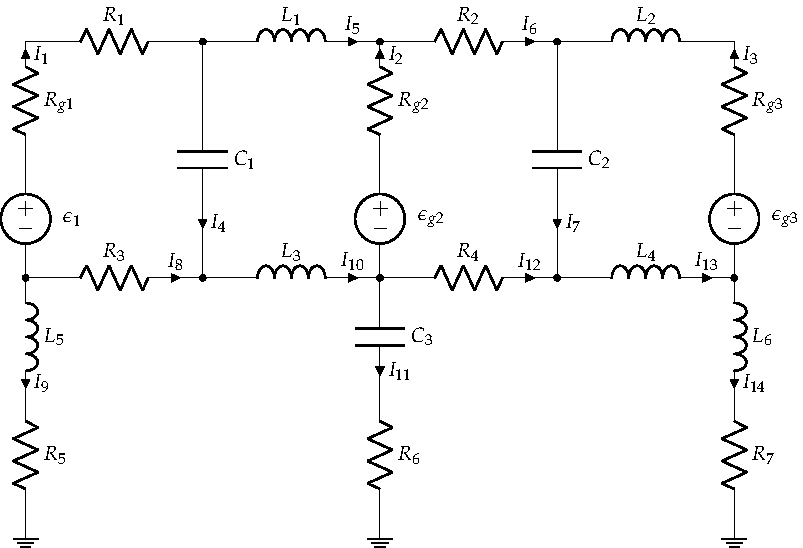
\includegraphics[scale = 0.8]{figs/mallas_condensadores_bobinas.pdf}
\end{minipage}

\subsection*{Solución}

Cuando el circuito se encuentra en régimen permanente, dado que las
fuentes son de corriente continua, los condensadores se sustituyen
por circuitos abiertos (inicialmente están descargados) y las bobinas
por cortocircuitos. De esta forma, el circuito original queda reducido
a tres mallas (A, B y C).

La resolución de este circuito mediante el método de las mallas se
sirve de la siguiente ecuación matricial:

\[
\left(\begin{array}{c}
E_{1}-E_{2}\\
E_{2}-E_{3}\\
0
\end{array}\right) = \left(\begin{array}{ccc}
R_{g1}+R_{1}+R_{g2}+R_{3} & -R_{g2} & -R_{3}\\
-R_{g2} & R_{g2}+R_{2}+R_{g3}+R_{4} & -R_{4}\\
-R_{3} & -R_{4} & R_{3}+R_{4}+R_{5}+R_{7}
\end{array}\right) \cdot \left(\begin{array}{c}
I_{A}\\
I_{B}\\
I_{C}
\end{array}\right)
\]
 y sustituyendo los valores de cada elemento:

\[
\left(\begin{array}{c}
18\\
2\\
0
\end{array}\right) = \left(\begin{array}{ccc}
12 & -4 & -2\\
-4 & 12 & -2\\
-2 & -2 & 6
\end{array}\right) \cdot \left(\begin{array}{c}
I_{A}\\
I_{B}\\
I_{C}
\end{array}\right)
\]
cuya solución es:

\begin{eqnarray*}
I_{A} & = & 2\, A\\
I_{B} & = & 1\, A\\
I_{C} & = & 1\, A
\end{eqnarray*}


Ahora debemos relacionar estas corrientes de malla con las corrientes
de rama señaladas en el circuito original (teniendo en cuenta que
las corrientes que circulan por ramas con condensadores son nulas):

\begin{eqnarray*}
I_{1} & = & I_{A}=2\, A\\
I_{2} & = & -I_{A}+I_{B}=-1\, A\\
I_{3} & = & -I_{B}=-1\, A\\
I_{4} & = & 0\, A\\
I_{5} & = & I_{A}=2\, A\\
I_{6} & = & I_{B}=1\, A\\
I_{7} & = & 0\, A\\
I_{8} & = & -I_{A}+I_{C}=-1\, A\\
I_{9} & = & -I_{C}=-1\, A\\
I_{10} & = & -I_{A}+I_{C}=-1\, A\\
I_{11} & = & 0\, A\\
I_{12} & = & -I_{B}+I_{C}=0\, A\\
I_{13} & = & -I_{B}+I_{C}=0\, A\\
I_{14} & = & I_{C}=1\, A
\end{eqnarray*}



\subsubsection*{Carga, polaridad y energía almacenada en los condensadores}


El condensador $C_{1}$ está conectado directamente a la rama compuesta
por la fuente $E_{2}$ y su resistencia $E_{g2}$ (debido a que la
bobina se comporta como un cortocircuito). Por tanto, suponiendo que
la polaridad positiva de este condensador corresponde a su borne superior,
la tensión de este condensador es:
\[
V_{C1}=E_{2}-I_{2}\cdot R_{g2}=22-(-1)\cdot4=26\, V
\]
siendo correcta la polaridad asignada por el signo positivo de este
resultado. La energía almacenada por el condensador es:
\[
E_{C1}=1/2\cdot V_{c1}^{2}\cdot C_{1}=0.676\, mJ
\]

El condensador $C_{2}$ está conectado directamente a la rama compuesta
por la fuente $E_{3}$ y su resistencia $E_{g3}$ (debido a que la
bobina se comporta como un cortocircuito). Por tanto, suponiendo que
la polaridad positiva de este condensador corresponde a su borne superior,
la tensión de este condensador es:
\[
V_{C2}=E_{3}-I_{3}\cdot R_{g3}=20-(-1)\cdot4=24\, V
\]
siendo correcta la polaridad asignada por el signo positivo de este
resultado. La energía almacenada por el condensador es:
\[
E_{C2}=1/2\cdot V_{c2}^{2}\cdot C_{2}=0.576\, mJ
\]


El condensador $C_{3}$ está en paralelo con la resistencia $R_{4}$
y la resistencia $R_{7}$ (debido a que las bobinas se comportan como
un cortocircuito y a que por la resistencia $R_{6}$ no circula corriente).
Por tanto, suponiendo que la polaridad positiva de este condensador
corresponde a su borne superior, la tensión de este condensador es:
\[
V_{C3}=I_{12}\cdot R_{4}+I_{14}\cdot R_{7}=0+1\cdot1=1\, V
\]
siendo correcta la polaridad asignada por el signo positivo de este
resultado. La energía almacenada por el condensador es:
\[
E_{C3}=1/2\cdot V_{c3}^{2}\cdot C_{3}=1\,\mu J
\]



\subsubsection*{Balance de potencias}


\begin{eqnarray*}
P_{E1} & = & E_{1}\cdot I_{1}=80\, W\\
P_{E2} & = & E_{2}\cdot I_{2}=-22\, W\\
P_{E3} & = & E_{3}\cdot I_{3}=-20\, W\\
P_{T} & = & P_{E1}+P_{E2}+P_{E3}=38\, W
\end{eqnarray*}


\begin{eqnarray*}
P_{Rg1} & = & I_{1}^{2}\cdot R_{g1}=16\, W\\
P_{Rg2} & = & I_{2}^{2}\cdot R_{g2}=4\, W\\
P_{Rg3} & = & I_{3}^{2}\cdot R_{g3}=4\, W\\
P_{R1} & = & I_{1}^{2}\cdot R_{1}=8\, W\\
P_{R2} & = & I_{6}^{2}\cdot R_{2}=2\, W\\
P_{R3} & = & I_{8}^{2}\cdot R_{3}=2\, W\\
P_{R4} & = & I_{12}^{2}\cdot R_{4}=0\, W\\
P_{R5} & = & I_{9}^{2}\cdot R_{5}=1\, W\\
P_{R6} & = & 0\, W\\
P_{R7} & = & I_{14}^{2}\cdot R_{7}=1\, W
\end{eqnarray*}
siendo que la suma de estas potencias individuales coincide con la
potencia total activa.

\clearpage

\section{}

En el circuito de la figura hay que determinar:

\begin{enumerate}
\item La corriente $i_1(t)$.
\item La potencia entregada por $e(t)$.
\item La potencia disipada por $R$.
\end{enumerate}

Datos: $R = \SI{5}{\ohm}$, $C = \SI{0.2}{\farad}$.

\subsection*{Solución}

\begin{enumerate}

\item La corriente $i(t)$.

  El período de las señales $i(t)$ y $e(t)$ es $T = \SI{2}{\second}$, por lo que los cálculos se realizan únicamente en el intervalo $0 \leq t < 2$.

Las expresiones analíticas de las señales de los generadores son:

\[
  e(t) = %
  \begin{cases}
    10\cdot t & 0 \leq t < 1\\
    20 - 10 \cdot t & 1 \leq t < 2 
  \end{cases}
\]

\[
  i(t) = %
  \begin{cases}
    -3 & 0 \leq t < 1\\
    3 & 1 \leq t < 2 
  \end{cases}
\]

Las expresiones de las corrientes del circuito son:

\[
  i_1(t) = i_c(t) - i(t)
\]

\[
  i_c(t) = C \diff{u_c(t)}{t} = C \diff{e(t)}{t}
\]



Derivamos $e(t)$ y obtenemos $i_c(t)$:

\[
  i_c(t) = %
  \begin{cases}
    2 & 0 \leq t < 1\\
    -2 & 1 \leq t < 2 
  \end{cases}
\]

A continuación descontamos la función $i(t)$ para obtener $i_1(t)$:

\[
  i_1(t) = %
  \begin{cases}
    5 & 0 \leq t < 1\\
    -5 & 1 \leq t < 2 
  \end{cases}
\]

\item La potencia entregada por $e(t)$.

  \begin{align*}
    p_E(t) &= e(t) \cdot i_1(t) = \\
           &=%
             \begin{cases}
               50\cdot t & 0 \leq t < 1\\
               50 \cdot t - 100 & 1 \leq t < 2 
             \end{cases}
  \end{align*}
  
  \begin{align*}
    P_E &= \frac{1}{T} \int_0^T p_E(t) \enspace \mathrm{dt}=\\
        &= \frac{1}{2} \left[ \int_0^1 10t \cdot 5 \enspace \mathrm{dt} + \int_1^2 (20 - 10t) \cdot (-5) \enspace \mathrm{dt}  \right] =\\
        &=\SI{0}{\watt}
  \end{align*}

  
\item La potencia disipada por $R$.

  \[
    P_R = R \cdot I^2
  \]

  $I$ es el valor eficaz de la corriente $i(t)$:

  \[
    I^2 = \frac{1}{T} \int_0^T i^2(t) \enspace \mathrm{dt} = 9
  \]

  \[
    P_R = \SI{45}{\watt}
  \]
  
\end{enumerate}

\clearpage

\section{}

En el circuito de la figura se pide:

\begin{enumerate}
\item Obtener la expresión analítica y la representación gráfica de las corrientes $i_L(t)$ e $i_R(t)$.
\item Calcular los valores medios y eficaces de las corrientes $i_L(t)$ e $i_R(t)$.
\item Obtener la expresión analítica y la representación gráfica de la corriente $i(t)$ y de la potencia del generador $e(t)$.
\end{enumerate}

Datos: $R = \SI{6}{\ohm}$, $L = \SI{4}{\milli\henry}$, $E = \SI{12}{\volt}$.

\subsection*{Solución}

\begin{enumerate}
\item $i_L(t)$ e $i_R(t)$
  Obtenemos la expresión analítica de $e(t)$ en el primer periodo de la señal ($T = \SI{2}{\milli\second}$):
  
  \[
    e(t) = %
    \begin{cases}
      12 & 0 \leq t < 10^{-3} \\
      -12 & 10^{-3} \leq t < 2 \cdot 10^{-3}
    \end{cases}
  \]

  A continuación obtenemos $i_R(t)$:

  \[
    i_R(t) = \frac{e(t)}{R} = %
    \begin{cases}
      2 & 0 \leq t < 10^{-3} \\
      -2 & 10^{-3} \leq t < 2 \cdot 10^{-3}
    \end{cases}
  \]

  Para obtener la corriente $i_L(t)$ debemos integrar por tramos, asumiendo que $i_L(-\infty) = 0$.

  \[
    i_L(t) = \frac{1}{L} \int_{-\infty}^t e(\tau) \enspace \mathrm{d}\tau = \frac{1}{L} \int_0^t e(\tau) \enspace \mathrm{d}\tau
  \]

  Calculamos esta integral por tramos:

  \begin{itemize}
  \item   $ 0 \leq t < 10^{-3}$
    \[
      i_L(t) = 250 \int_0^t 12 \enspace \mathrm{d}\tau = 3\cdot 10^3 \cdot t
    \]
    Particularizamos en los extremos temporales:
    
    \begin{align*}
      i_L(t = 0) &= \SI{0}{\ampere}\\
      i_L(t = 10^{-3}) &= \SI{3}{\ampere}
    \end{align*}
    
  \item $10^{-3} \leq t < 2 \cdot 10^{-3}$
    \[
      i_L(t = 10^{-3}) + 250 \int_{10^{-3}}^t -12 \enspace \mathrm{d}\tau = 3 + 3\cdot 10^3 \cdot (10^{-3} - t) = 6- 3 \cdot 10^3 \cdot t
    \]

    Particularizamos:
    \begin{align*}
      i_L(t = 10^{-3}) &= \SI{3}{\ampere}\\
      i_L(t = 2 \cdot 10^{-3}) &= \SI{0}{\ampere}
    \end{align*}

  \end{itemize}

  
\item Valores medios y eficaces.

  El valor medio de $i_R(t)$ es 0. Calculamos el valor medio en un semiperiodo:

  \[
    I_{Rm}(t) = \frac{2}{T} \int_0^{T/2} i_R(t) \enspace \mathrm{dt} = \SI{2}{\ampere} 
  \]

  El valor eficaz de esta señal coincide con su valor máximo.

  \[
    I_R(t) = \sqrt{\frac{1}{T} \int_0^T i^2_R(t) \enspace \mathrm{dt}} = \SI{2}{\ampere} 
  \]

  Para la corriente $i_L(t)$ aprovechamos su simetría y calculamos únicamente en un semiperiodo:

    \[
      I_{Lm}(t) = \frac{1}{T} \int_0^{T/2} i_L(t) \enspace \mathrm{dt} = 10^3 \int_0^{10^{-3}} 3 \cdot 10 ^3 \cdot t \enspace \mathrm{dt} = \SI{1.5}{\ampere} 
  \]

      \[
      I^2_L(t) = \frac{1}{T} \int_0^{T/2} i^2_L(t) \enspace \mathrm{dt} = 10^3 \int_0^{10^{-3}} (3 \cdot 10 ^3 \cdot t)^2 \enspace \mathrm{dt} = 3 \Rightarrow I_L = \SI{1.5}{\ampere} 
  \]

  
\item $i(t)$ y $p_E(t)$

  \[
    i(t) = i_R(t) + i_L(t)
  \]

  \[
    i(t) = %
    \begin{cases}
      2 + 3\cdot 10^3 \cdot t &  0 \leq t < 10^{-3}\\ 
      4 - 3\cdot 10^3 \cdot t & 10^{-3} \leq t < 2 \cdot 10^{-3}
    \end{cases}
  \]

  \[
    p_E(t) = e(t) \cdot i(t)
  \]
  
  \[
    p_E(t) = %
    \begin{cases}
      24 + 36\cdot 10^3 \cdot t &  0 \leq t < 10^{-3}\\ 
      -48 + 36\cdot 10^3 \cdot t & 10^{-3} \leq t < 2 \cdot 10^{-3}
    \end{cases}
  \]

\end{enumerate}

\end{document}





